\documentclass{amsart} 
\usepackage{graphicx}
\graphicspath{{./}}
\usepackage[fontsize=14pt]{scrextend}
\usepackage{hyperref}
\usepackage{csvsimple}
\usepackage{epigraph}
\title{Is Work Duty Towards Society?}
\author{Zulfikar Moinuddin Ahmed}
\date{\today}
\begin{document}
\maketitle

\section{What is Society?}
I would consider myself an expert on the issue of {\em definition} of society.  See today I am American, with 33 years in America of which 23 years I have been a Permanent Resident. 

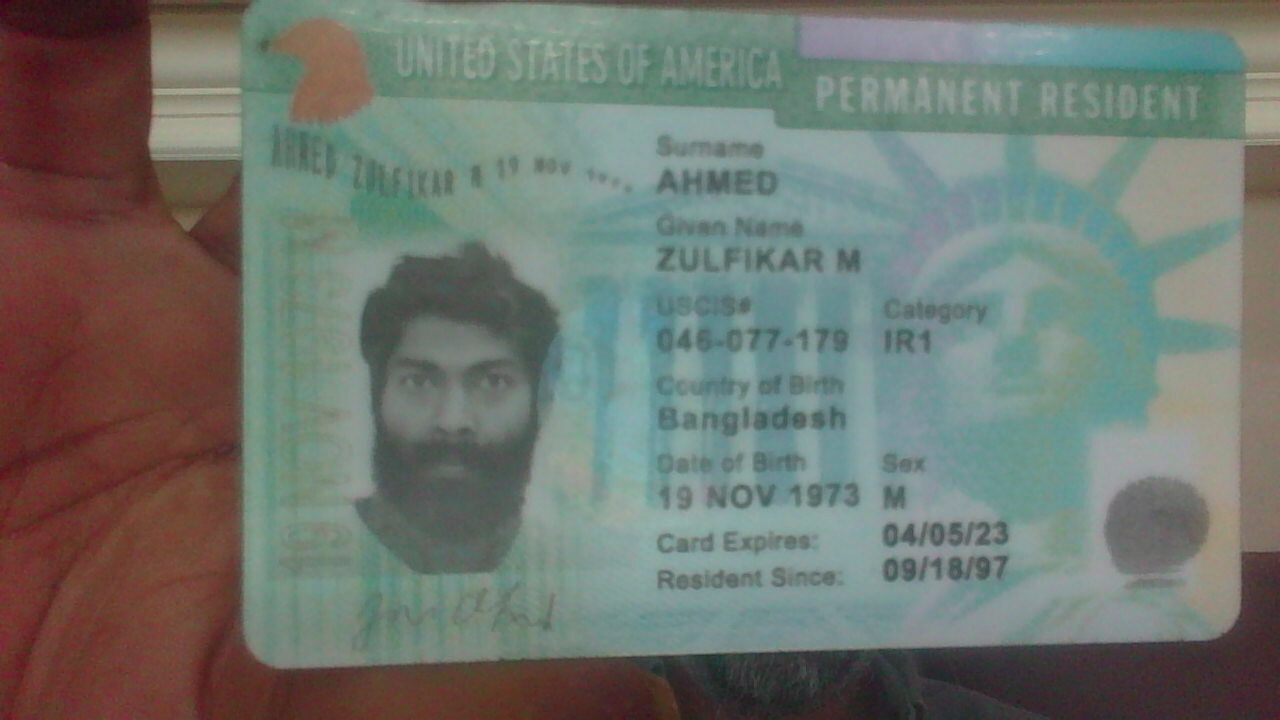
\includegraphics[scale=0.26]{gc.png}

But I had a complicated and unstable childhood in Bengal and my puberty and adolescence was in New York.  My father never moved to America and was very senior in civil service and found meaning in his life in service to Bengali people.  I studied Mathematics at Princeton and entered Industry in Finance in 1995.  In the process of personal evolution I accepted not just American people as my own, but had also to expand my people to the entire Human Race.  There are of course reasons for that, and influences, such as my anti-war protests during Iraq War with my colleagues in International Socialist Organization in 2003-4.  In any case, the strong end of the process is decision that Human Race is a Single Race, despite nationalist enthusiasm in the past decade including much work to ensure correctness of the Scientific position on Single Human Race. For me Society is the Human Race and not a city or even just American Society.

And this is the crucial thing for me.  Unless Society is the Human Race, I have little satisfaction considering my work as duty to Society.  I am Zulf.  I am expansive and vast.  To me 'duty to society' is too clautrophobic if it is just for a nation.  I would lose motivation and become anxious and unsatisfied.  But once Society is Human Race, then I am willing to consider Work as a delightful Duty to Society.  Then I don't feel as much burden.

\section{Distribution}

This is the distribution of percentages across $N=70$ countries who do not believe work is a duty to society.

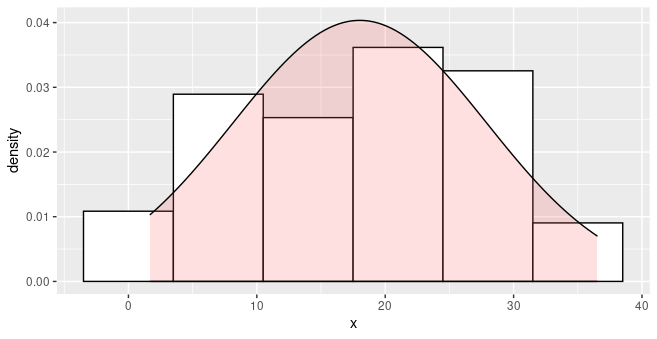
\includegraphics[scale=0.7]{wnduty.png}

The mean is 18\%.  Unless I defined Society as Human Race, I would fall in this minority.

This is a truly interesting issue because there is a temptation to consider naturally that it is Human Nature to consider work as duty to society and explain the deviation to make precise sense of  the parameters that ought to be included as human nature.

\end{document}